\documentclass[11pt]{report}

\usepackage{tocloft}
\usepackage{epsf,amsmath,amsfonts}
\usepackage{graphicx}
\usepackage{longtable}
\usepackage[pagebackref=true]{hyperref}
\usepackage{color}
\usepackage[hang]{caption}
%\usepackage[hang]{subfigure}
\usepackage{subfig}
\usepackage{natbib}
\usepackage{placeins}
\usepackage{eso-pic}
\usepackage{float}

\definecolor{black}{rgb}{0.0,0.0,0.0}
\definecolor{darkblue}{rgb}{0.0,0.0,0.5}
\hypersetup{colorlinks,breaklinks,
            linkcolor=blue,urlcolor=blue,
            anchorcolor=black,citecolor=blue}
			

\renewcommand\cftsecaftersnumb{
\,\,
}
\renewcommand\cftsubsecaftersnumb{
\,\,
}
\renewcommand\cftsubsubsecaftersnumb{
\,\,
}

\setlength{\topmargin}{0in}
\setlength{\headheight}{0in}
\setlength{\headsep}{0in}
\setlength{\textheight}{9.0in}
\setlength{\textwidth}{6.5in}
\setlength{\evensidemargin}{0in}
\setlength{\oddsidemargin}{0in}

%\captionsetup{width=2in}
\captionsetup{format=hang}
%\captionsetup{justification=RaggedRight}

%\newcommand{\version}{1.3}


\setlength\LTleft\parindent
\setlength\LTright\fill

\newcommand\BackgroundPic{%
	\put(0,0){%
		\parbox[b][\paperheight]{\paperwidth}{%
			\centering
			
\includegraphics[width=\paperwidth,height=\paperheight,keepaspectratio]{ocean/figures/MPAS_LOGO_Ocean.png}%
			\vfill
			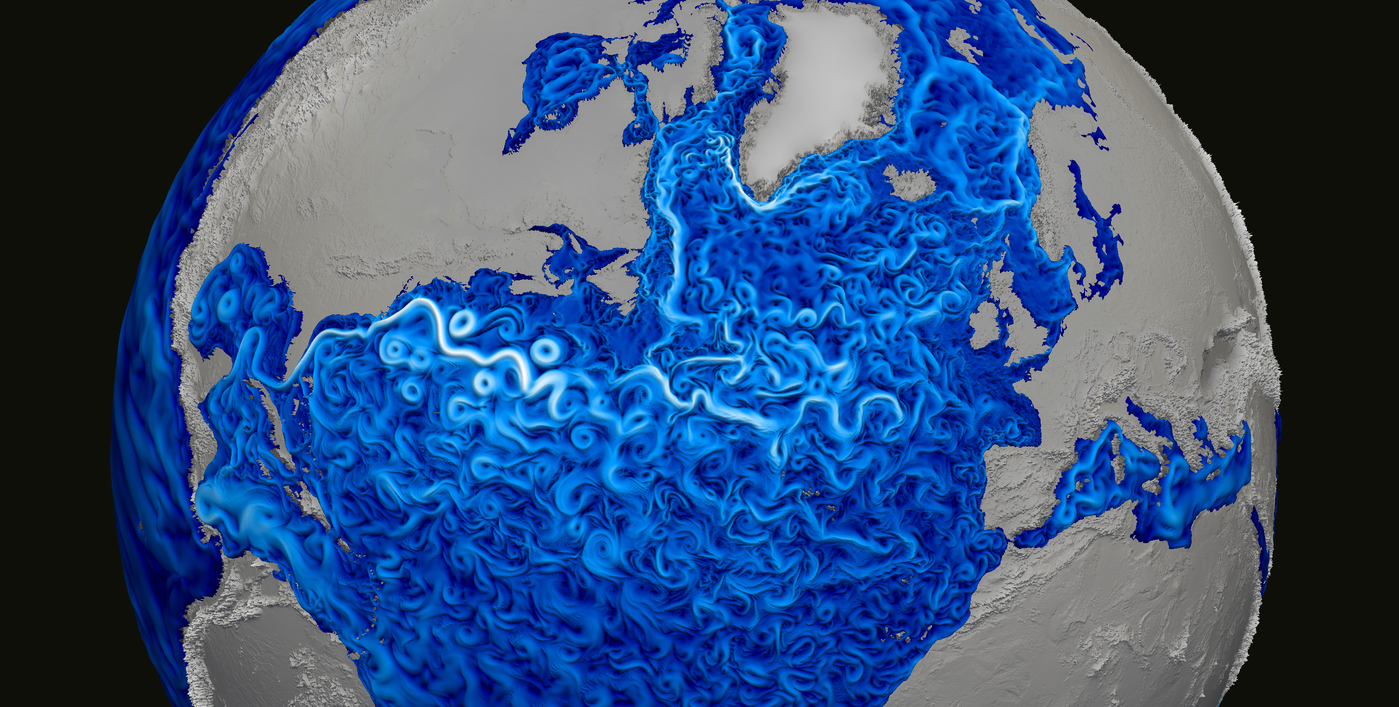
\includegraphics[width=\paperwidth,height=\paperheight,keepaspectratio]{ocean/figures/cover_V3_KE_NA37-7km_cropped_d.png}%
}}}

\newcommand{\inlineCode}[1]{\textbf{#1}}

\newcommand{\core}{seaice}

\begin{document}
%\AddToShipoutPicture*{\BackgroundPic}

\title{
\Huge MPAS-Seaice Model User's Guide \\
%\LARGE Version: \version
}

\author{
\LARGE Climate, Ocean, Sea-Ice Modeling Team\\ \\
\LARGE Los Alamos National Laboratory
}

\date{PUT RELEASE DATE HERE May 1, 2018}

\maketitle

\chapter*{Copyright}
\label{chap:copyright}
{\bf Copyright \copyright 2013,  Los Alamos National Security, LLC (LANS) (LA-CC-13-047)
and the University Corporation for Atmospheric Research (UCAR).} \\

All rights reserved.  \\

LANS is the operator of the Los Alamos National Laboratory under Contract No.
DE-AC52-06NA25396 with the U.S. Department of Energy.  UCAR manages the National
Center for Atmospheric Research under Cooperative Agreement ATM-0753581 with the
National Science Foundation.  The U.S. Government has rights to use, reproduce,
and distribute this software.  NO WARRANTY, EXPRESS OR IMPLIED IS OFFERED BY
LANS, UCAR OR THE GOVERNMENT AND NONE OF THEM ASSUME ANY LIABILITY FOR THE USE
OF THIS SOFTWARE.  If software is modified to produce derivative works, such
modified software should be clearly marked, so as not to confuse it with the
version available from LANS and UCAR. \\

Additionally, redistribution and use in source and binary forms, with or without
modification, are permitted provided that the following conditions are met: \\

1) Redistributions of source code must retain the above copyright notice, this
list of conditions and the following disclaimer. \\

2) Redistributions in binary form must reproduce the above copyright notice,
this list of conditions and the following disclaimer in the documentation and/or
other materials provided with the distribution. \\

3) None of the names of LANS, UCAR or the names of its contributors, if any, may
be used to endorse or promote products derived from this software without
specific prior written permission. \\

THIS SOFTWARE IS PROVIDED BY THE COPYRIGHT HOLDERS AND CONTRIBUTORS "AS IS" AND
ANY EXPRESS OR IMPLIED WARRANTIES, INCLUDING, BUT NOT LIMITED TO, THE IMPLIED
WARRANTIES OF MERCHANTABILITY AND FITNESS FOR A PARTICULAR PURPOSE ARE
DISCLAIMED. IN NO EVENT SHALL THE COPYRIGHT HOLDER OR CONTRIBUTORS BE LIABLE FOR
ANY DIRECT, INDIRECT, INCIDENTAL, SPECIAL, EXEMPLARY, OR CONSEQUENTIAL DAMAGES
(INCLUDING, BUT NOT LIMITED TO, PROCUREMENT OF SUBSTITUTE GOODS OR SERVICES;
LOSS OF USE, DATA, OR PROFITS; OR BUSINESS INTERRUPTION) HOWEVER CAUSED AND ON
ANY THEORY OF LIABILITY, WHETHER IN CONTRACT, STRICT LIABILITY, OR TORT
(INCLUDING NEGLIGENCE OR OTHERWISE) ARISING IN ANY WAY OUT OF THE USE OF THIS
SOFTWARE, EVEN IF ADVISED OF THE POSSIBILITY OF SUCH DAMAGE.
\newpage


\tableofcontents

\part{The MPAS Framework}
\chapter{Building MPAS}
\label{chap:mpas_build_instructions}

\section{Prequisites}

To build MPAS, compatible C and Fortran compilers are required. Additionally, the MPAS software relies on the PIO parallel I/O library to read and write model fields, and the PIO library requires the standard netCDF library as well as the parallel-netCDF library from Argonne National Labs. All libraries must be compiled with the same compilers that will be used to build MPAS. Section \ref{sec:build_io} summarizes the basic procedure of installing the required I/O libraries for MPAS.

In order for the MPAS makefiles to find the PIO, parallel-netCDF, and netCDF include files and libraries, the environment variables {\tt PIO}, {\tt PNETCDF}, and {\tt NETCDF} should be set to the root installation directories of the PIO, parallel-netCDF, and netCDF installations, respectively. Newer versions of the netCDF library use a separate Fortran interface library; the top-level MPAS Makefile attempts to add {\tt -lnetcdff} to the linker flags, but some linkers require that {\tt -lnetcdff} appear before {\tt -lnetcdf}, in which case {\tt -lnetcdff} will need to be manually added just before {\tt -lnetcdf} in the specification of {\tt LIBS} in the top-level Makefile.

An MPI installation such as MPICH or OpenMPI is also required, and there is no option to build a serial version of the MPAS executables. There is currently no support for shared-memory parallelism with OpenMP within the MPAS framework.


\section{Compiling I/O Libraries}
\label{sec:build_io}

{\bf NOTE:} It's important to note the MPAS Developers are not responsible for any of the libraries that are used within MPAS. Support for specific libraries should be taken up with the respective developer groups.

Although most recent versions of the I/O libraries should work, the most tested versions of these libraries are: netCDF 4.1.3, parallel-netCDF 1.3.1, and PIO 1.4.1. The netCDF and parallel-netCDF libraries must be installed before building PIO library.

All commands are presented for csh, and will not work if pasted into another shell. Please translate them to the appropraite commands in your shell.

\subsection{netCDF}

Version 4.1.3 of the netCDF library may be downloaded from \url{http://www.unidata.ucar.edu/downloads/netcdf/netcdf-4\_1\_3/index.jsp}.
Assuming the gfortran and gcc compilers will be used, the following shell commands are generally sufficient to install netCDF.

\vspace{12pt}
{\tt > setenv FC gfortran}

{\tt > setenv F77 gfortran} 

{\tt > setenv F90 gfortran}

{\tt > setenv CC gcc} 

{\tt > ./configure --prefix=XXXXX --disable-dap --disable-netcdf-4 --disable-cxx \hfill\break --disable-shared --enable-fortran} 

{\tt > make all check}

{\tt > make install}
\vspace{12pt}

Here, {\tt XXXXX} should be replaced with the directory that will serve as the root installation directory for netCDF.
{\em Before proceeding to compile PIO the {\tt NETCDF\_PATH} environment variable should be set to the netCDF root installation directory.}

Certain compilers require addition flags in the CPPFLAGS environment variable. Please refer to the netCDF installation instructions for these flags.

\subsection{parallel-netCDF}

Version 1.3.1 of the parallel-netCDF library may be downloaded from \url{https://trac.mcs.anl.gov/projects/parallel-netcdf/wiki/Download}.
Assuming the gfortran and gcc compilers will be used, the following shell commands are generally sufficient to install parallel-netCDF.

\vspace{12pt}
{\tt > setenv MPIF90 mpif90}

{\tt > setenv MPIF77 mpif90} 

{\tt > setenv MPICC mpicc}  

{\tt > ./configure --prefix=XXXXX} 

{\tt > make}

{\tt > make install}
\vspace{12pt}

Here, {\tt XXXXX} should be replaced with the directory that will serve as the root installation directory for parallel-netCDF.
{\em Before proceeding to compile PIO the {\tt PNETCDF\_PATH} environment variable should be set to the parallel-netCDF root installation directory.}


\subsection{PIO}

Instructions for building PIO can be found at \url{http://www.cesm.ucar.edu/models/pio/}. Please refer to these instructions for building PIO.

After PIO is built, and installed the PIO enviroment variable needs to be
defined to point at the directory PIO is installed into. Older versions of PIO
cannot be installed, and the PIO environment variable needs to be set to the
directory where PIO was built instead.

\section{Compiling MPAS}

{\bf \em Before compiling MPAS, the {\tt NETCDF}, {\tt PNETCDF}, and {\tt PIO} environment variables must be set to the library installation directories as
described in the previous section. A {\tt CORE} variable also needs to either be defined or passed in during the make process. If {\tt CORE} is not specified, 
the build process will fail.}

The MPAS code uses only the `make' utility for compilation. Rather than employing a separate configuration step
before building the code, all information about compilers, compiler flags, etc., is contained in the top-level {\tt Makefile}; each
supported combination of compilers (i.e., a configuration) is included in the {\tt Makefile} as a separate make target, and the user selects among
these configurations by running {\tt make} with the name of a build target specified on the command-line, e.g.,

\vspace{12pt}
{\tt > make gfortran}
\vspace{12pt}

\noindent to build the code using the GNU Fortran and C compilers. Some of the available targets are listed in the table below, and additional
targets can be added by simply editing the {\tt Makefile} in the top-level directory.

\vspace{12pt}
\begin{longtable}{| l | l | l | l |}
\hline
Target & Fortran compiler & C compiler & MPI wrappers \\ \hline \hline
{\tt xlf} & xlf90 & xlc & mpxlf90 / mpcc \\ \hline
{\tt pgi} & pgf90 & pgcc & mpif90 / mpicc \\ \hline
{\tt ifort} & ifort & gcc & mpif90 / mpicc \\ \hline
{\tt gfortran} & gfortran & gcc & mpif90 / mpicc \\ \hline
{\tt g95} & g95 & gcc & mpif90 / mpicc \\ \hline
\end{longtable}
\vspace{12pt}

In order to get a more complete and up-to-date list of available tagets, one can use the following command within the top-level of MPAS. {\bf NOTE: }This command is known to not work with Mac OSX.
{\small
\begin{verbatim}
> make -rpn | sed -n -e '/^$/ { n ; /^[^ ]*:/p }' | sed "s/: *.*$//g"
\end{verbatim}
}

The MPAS framework supports multiple {\em cores} --- currently a shallow water
model, an ocean model, a non-hydrostatic atmosphere model, and a non-hydrostatic atmosphere initialization core --- so the build
process must be told which core to build. This is done by either setting the environment variable
{\tt CORE} to the name of the model core to build, or by specifying the core to be built explicitly on the command-line
when running {\tt make}. For the shallow water core, for example, one may run either

\vspace{12pt}
{\tt > setenv CORE sw}

{\tt > make gfortran}
\vspace{12pt}

\noindent or

\vspace{12pt}
{\tt > make gfortran CORE=sw}
\vspace{12pt}

If the {\tt CORE} environment variable is set and a core is specified on the command-line, the command-line value takes precedence; if no core
is specified, either on the command line or via the {\tt CORE} environment variable, the build process will stop with an error message stating such.
Assuming compilation is successful, the model executable, named {\tt \$\{CORE\}\_model.exe} (e.g., {\tt sw\_model.exe}), should
be created in the {\tt src/} subdirectory, and a symbolic link to the model executable 
should exist in the top-level MPAS directory.

In order to get a list of available cores, one can simply run the top-level {\tt Makefile} without setting the {\tt CORE} environment variable, or passing the core via the command-line. And example of the output from this can be seen below.

{\small
\begin{verbatim}
> make
( make error )
make[1]: Entering directory `/home/douglasj/Documents/svn-mpas-model.cgd.ucar.edu/trunk/mpas'

Usage: make target CORE=[core] [options]

Example targets:
ifort
gfortran
xlf
pgi

Availabe Cores:
atmosphere
init_atmosphere
ocean
sw

Available Options:
DEBUG=true    - builds debug version. Default is optimized version.
USE_PAPI=true - builds version using PAPI for timers. Default is off.
TAU=true      - builds version using TAU hooks for profiling. Default is off.

Ensure that NETCDF, PNETCDF, PIO, and PAPI (if USE_PAPI=true) are environment variables
that point to the absolute paths for the libraries.

************ ERROR ************
No CORE specified. Quitting.
************ ERROR ************

make[1]: Leaving directory `/home/douglasj/Documents/svn-mpas-model.cgd.ucar.edu/trunk/mpas'
\end{verbatim}
}

\section{Cleaning}

To remove all files  that were created when the model was built, including the model executable itself, {\tt make} may
be run for the `clean' target:

\vspace{12pt}
{\tt > make clean}
\vspace{12pt}

As with compiling, the core to be cleaned is specified by the {\tt CORE} environment variable, or by specifying a core explicitly on the command-line with {\tt CORE=}.


\section{Graph partitioning with METIS} 
\label{sec:metis}

% this section is also in mpas_grid_generation.tex.  When grid generation is included in a future release, delete this section from this chapter.

Before MPAS can be run in parallel, a mesh decomposition file with an appropriate number of 
partitions (equal to the number of MPI tasks that will be used) is required in the run directory.  A limited number of mesh decomposition files ({\tt graph.info.part.*}) are provided with each test case.  In order to create new mesh decomposition files for your desired number of partitions, begin with the provided {\tt graph.info} file and partition with METIS software (\url{http://glaros.dtc.umn.edu/gkhome/views/metis}). The serial graph partitioning program, METIS (rather than ParMETIS or hMETIS) should be sufficient for quickly partitioning any SCVT produced by the grid\_gen mesh generator.

After installing METIS, a {\tt graph.info} file may be partitioned into $N$ partitions by running

\vspace{12pt}
{\tt > gpmetis graph.info} $N$
\vspace{12pt}

\noindent The resulting file, {\tt graph.info.part.}$N$, can then be copied into the MPAS run directory
before running the model with $N$ MPI tasks.

\chapter{Grid Description}
\label{chap:mpas_grid_description}

This chapter provides a brief introduction to the common types of grids used in the MPAS framework. 

The MPAS grid system requires the definition of seven elements. These seven elements are composed of two types of {\it cells}, two types of {\it lines}, and three types of {\it points}. These elements are depicted in Figure \ref{figure:variablePosition} and defined in Table \ref{table:variablePosition}.  These elements can be defined on either the plane or the surface of the sphere. The two types of cells form two meshes, a primal mesh composed of Voronoi regions and a dual mesh composed of Delaunay triangles. Each corner of a primal mesh cell is uniquely associated with the ``center'' of a dual mesh cell and vice versa. So we define the two mesh as either a primal mesh (composed of cells $P_i$) or a dual mesh (composed of cells $D_v$). The center of any primal mesh cell, $P_i$, is denoted by ${\bf x}_i$ and the center of any the dual mesh cell, $D_v$, is denoted by ${\bf x}_v$. The boundary of a given primal mesh cell $P_i$ is composed of the set of lines that connect the ${\bf x}_v$ locations of associated dual mesh cells $D_v$. Similarly, the boundary of a given dual mesh cell $D_v$ is composed of the set of lines that connect the ${\bf x}_i$ locations of the associated primal mesh cells $P_i$. 

As shown in Figure \ref{figure:variablePosition}, a line segment that connects two primal mesh cell centers is uniquely associated with a line segment that connects two dual mesh cell centers. We assume that these two line segments cross and the point of intersection is labeled as ${\bf x}_e$. In addition, we assume that these two line segments are orthogonal as indicated in Figure \ref{figure:variablePosition}. Each ${\bf x}_e$ is associated with two distances: $d_e$ measures the distance between the primal mesh cells sharing ${\bf x}_e$ and $l_e$ measures the distance between the dual mesh cells sharing ${\bf x}_e$.

Since the two line segments crossing at ${\bf x}_e$ are orthogonal, these line segments form a convenient local coordinate system for each edge. At each ${\bf x}_e$ location a unit vector ${\bf n}_e$ is defined to be parallel to the line connecting primal mesh cells. A second unit vector ${\bf t}_e$ is defined such that ${\bf t}_e = {\bf k} \times {\bf n}_e$.

In addition to these seven element types, we require the definition of {\it sets of elements}. In all, eight different types of sets are required and these are defined and explained in Table \ref{table:gridConnectivity} and Figure \ref{figure:gridConnectivity}. The notation is always of the form of, for example, $i \in CE(e)$, where the LHS indicates the type of element to be gathered (cells) based on the RHS relation to another type of element (edges).

Table \ref{table:gridFileName} provides the names of all {\it elements} and all {\it sets of elements} as used in the MPAS framework.  Elements appear twice in the table when described in the grid file in more than one way, e.g. points are described with both cartesian and latitude/longitude coordinates. An ``ncdump -h'' of any MPAS grid, output or restart file will contain all variable names shown in second column of Table  \ref{table:gridFileName}.


\begin{table}[t]
\caption{Definition of elements used to build the MPAS grid.}
\label{table:variablePosition}
\begin{center}
\begin{tabular}{lll}
\hline\hline
$Element$ & $Type$ & $Definition$\\
\hline
 ${\bf x}_i$   & point             & location of center of primal-mesh cells \\
 ${\bf x}_v$  &  point            & location of center of dual-mesh cells \\
 ${\bf x}_e$  & point             & location of edge points where velocity is defined \\
 $d_{e}$       & line segment & distance between neighboring ${\bf x}_i$ locations \\
 $l_{e}$       & line segment & distance between neighboring ${\bf x}_v$ locations \\
 $P_i$         & cell                 & a cell on the primal-mesh \\
 $D_v$        & cell                 & a cell on the dual-mesh \\
\hline
\end{tabular}
\end{center}
\end{table}
%
\begin{table}[t]
\caption{Definition of element groups used to reference connections in the MPAS grid. Examples are provided in Figure \ref{figure:gridConnectivity}.}
\label{table:gridConnectivity}
\begin{center}
\begin{tabular}{lll}
\hline\hline
$Syntax$ & $ouptut$\\
\hline
 $e \in EC(i) $   & set of edges that define the boundary of $P_i$. \\
 $e \in EV(v) $     & set of edges that define the boundary of $D_v$. \\
 $i \in CE(e) $                 & two primal-mesh cells that share edge $e$. \\
 $i \in CV(v) $  &  set of primal-mesh cells that form the vertices of dual mesh cell $D_v$. \\
 $v\in VE(e) $  & the two dual-mesh cells that share edge $e$. \\
 $v \in VI(i) $   & the set of dual-mesh cells that form the vertices of primal-mesh cell $P_i$. \\
 $e \in ECP(e)$ & edges of cell pair meeting at edge $e$. \\
 $e \in EVC(v,i)$ & edge pair associated with vertex $v$ and mesh cell $i$. \\
\hline
\end{tabular}
\end{center}
\end{table}
%

\begin{table}[t]
\caption{Variable names used to describe a MPAS grid.}
\label{table:gridFileName}
\begin{center}
\begin{tabular}{llll}
\hline\hline
$Element$ & $Name$ & $Size$ & $Comment$\\
\hline
 ${\bf x}_i$   & \{x,y,z\}Cell          & nCells  & cartesian location of ${\bf x}_i$  \\
 ${\bf x}_i$   & \{lon,lat\}Cell        & nCells  & longitude and latitude of  ${\bf x}_i$  \\
 ${\bf x}_v$   & \{x,y,z\}Vertex      & nVertices  & cartesian location of ${\bf x}_v$  \\
 ${\bf x}_v$   & \{lon,lat\}Vertex    & nVertices  & longitude and latitude of  ${\bf x}_v$  \\
 ${\bf x}_e$   & \{x,y,z\}Edge          & nEdges  & cartesian location of ${\bf x}_e$  \\
 ${\bf x}_e$   & \{lon,lat\}Edge        & nEdges  & longitude and latitude of  ${\bf x}_e$  \\
 $d_{e}$       & dcEdge                   & nEdges  & distance between ${\bf x}_i$ locations\\
 $l_{e}$         & dvEdge             & nEdges &  distance between ${\bf x}_v$ locations \\
  &  & & \\
 $e \in EC(i) $   &  edgesOnCell  & (nEdgesMax,nCells) & edges that define $P_i$. \\
 $e \in EV(v) $     & edgesOnVertex &  (3,nCells) & edges that define $D_v$. \\
 $i \in CE(e) $      & cellsOnEdge &  (2,nEdges) &  primal-mesh cells that share edge $e$. \\
 $i \in CV(v) $  &   cellsOnVertex &  (3,nVertices) &  primal-mesh cells that define $D_v$. \\
 $v\in VE(e) $  & verticesOnEdge &  (2,nEdges) &    dual-mesh cells that share edge $e$. \\
 $v \in VI(i) $   & verticesOnCell &  (nEdgesMax,nCells) & vertices that define $P_i$. \\
\hline
\end{tabular}
\end{center}
\end{table}
%


%
\begin{figure}[t]
  \noindent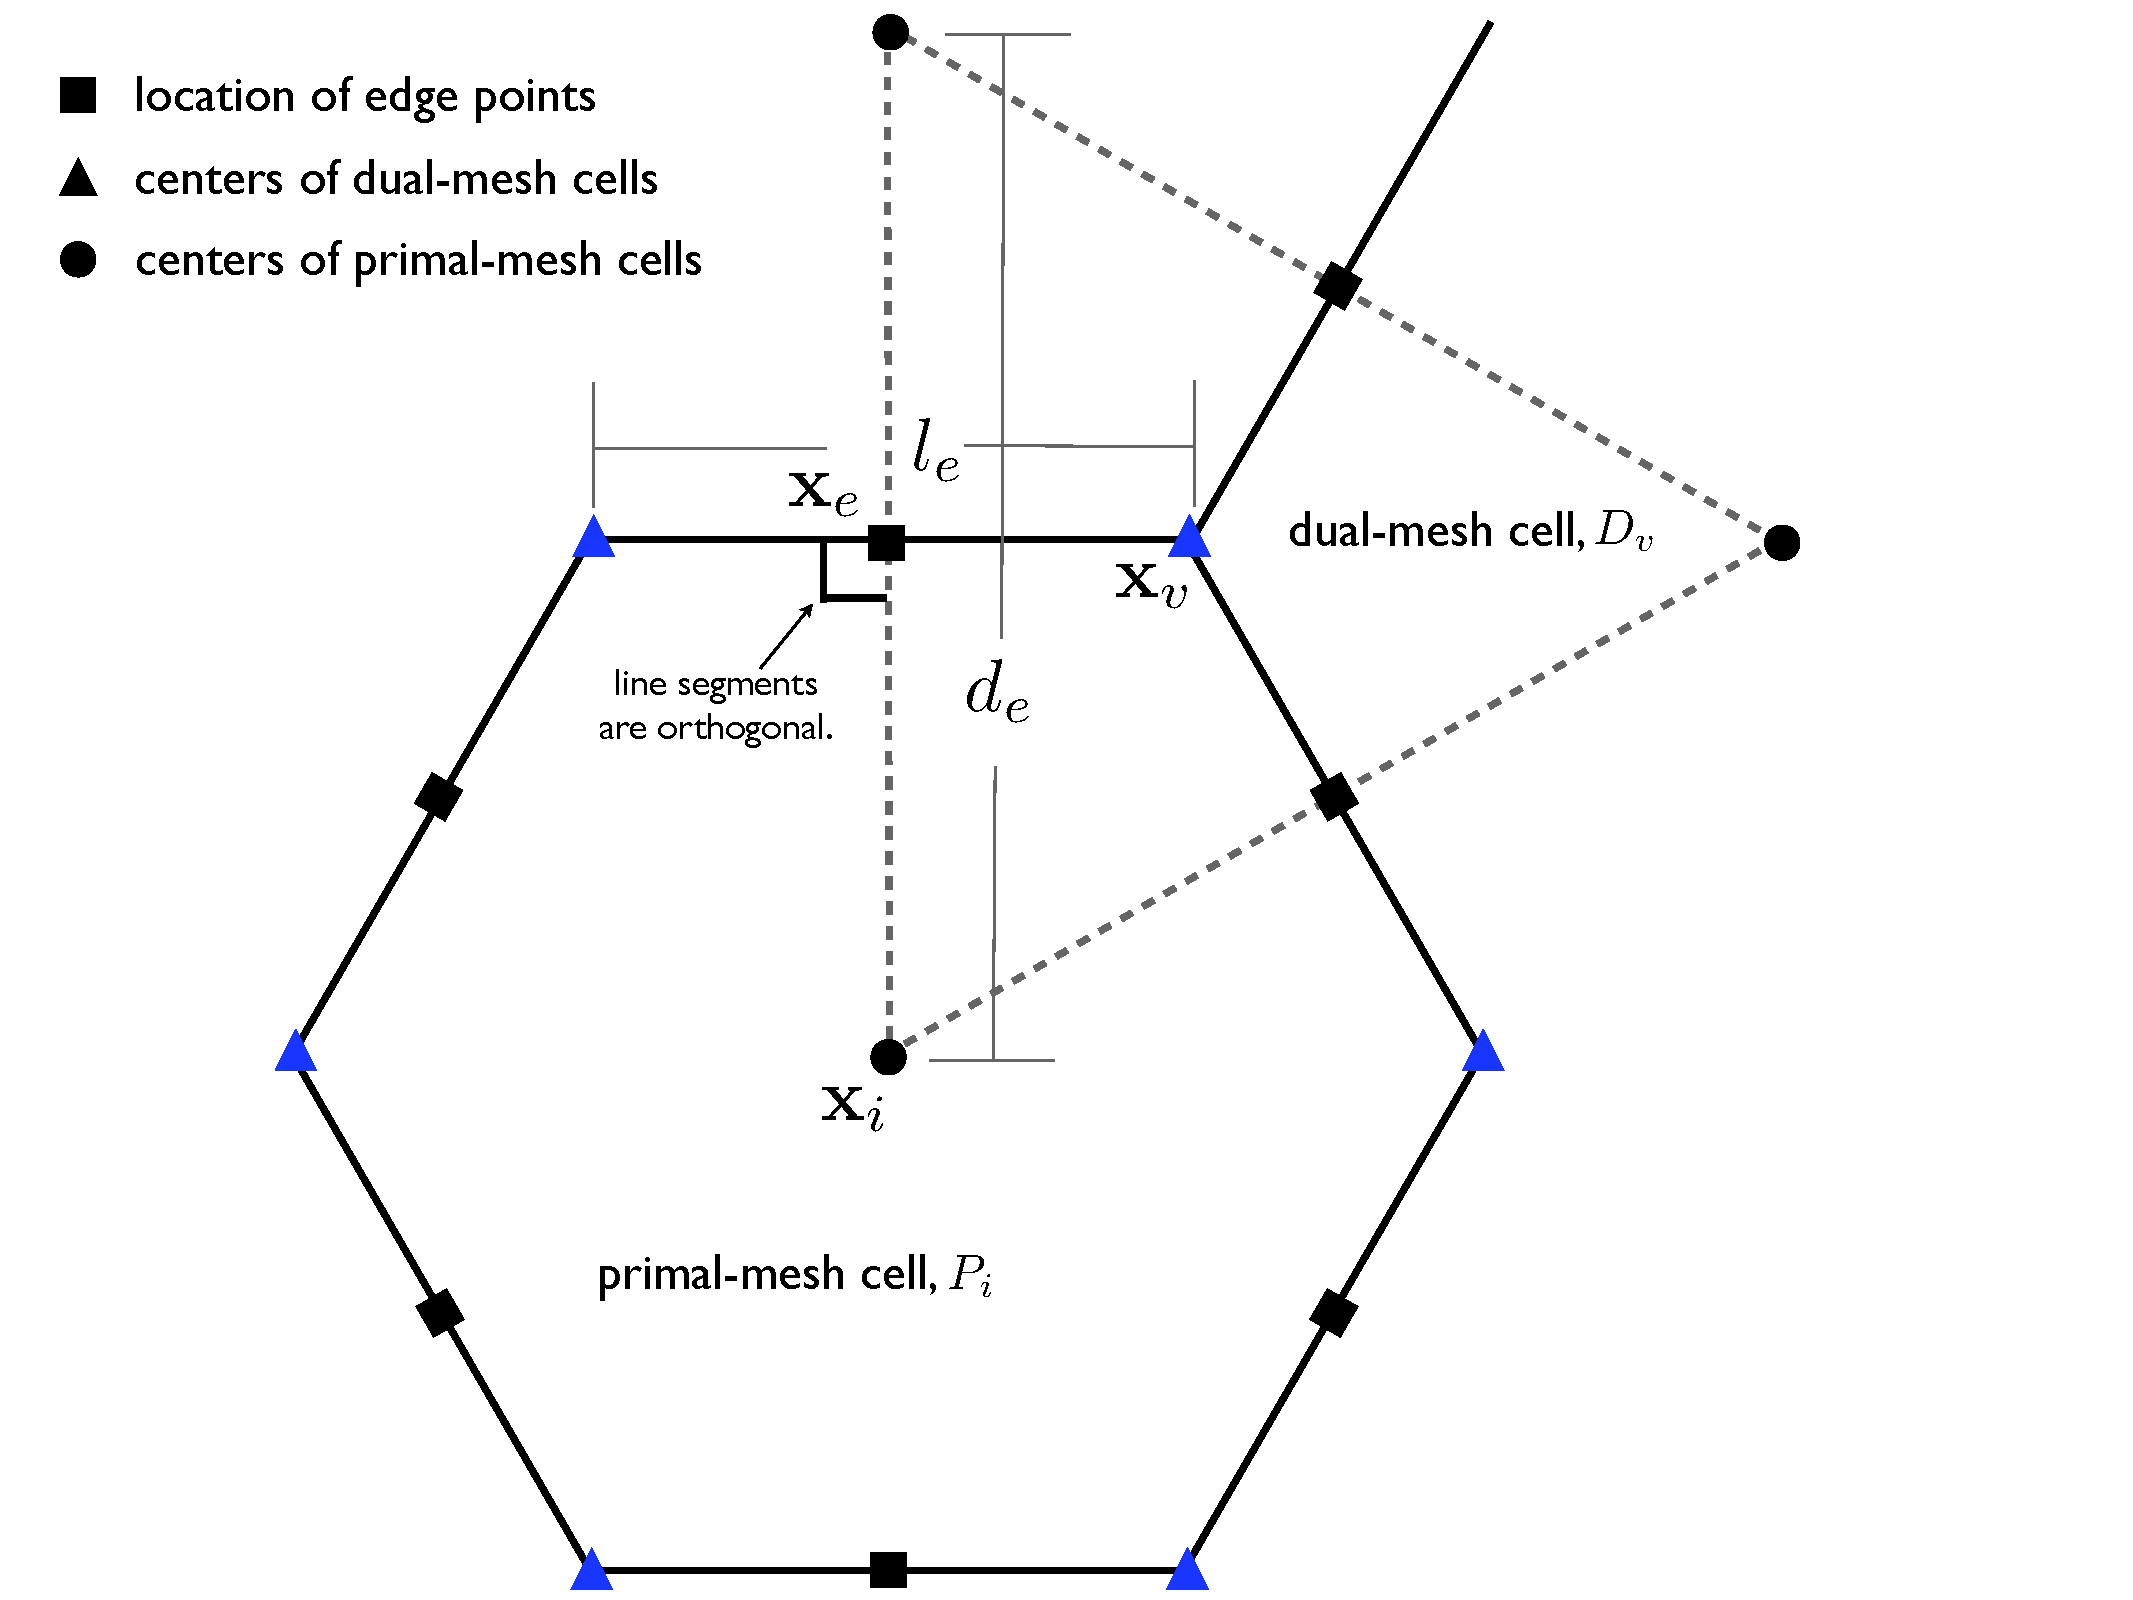
\includegraphics[width=16cm,angle=0]{./shared/figures/variablePosition.pdf}\\
  \caption{Definition of elements used to build the MPAS grid. Also see Table \ref{table:variablePosition}.}
  \label{figure:variablePosition}
\end{figure}

%
\begin{figure}[t]
   \noindent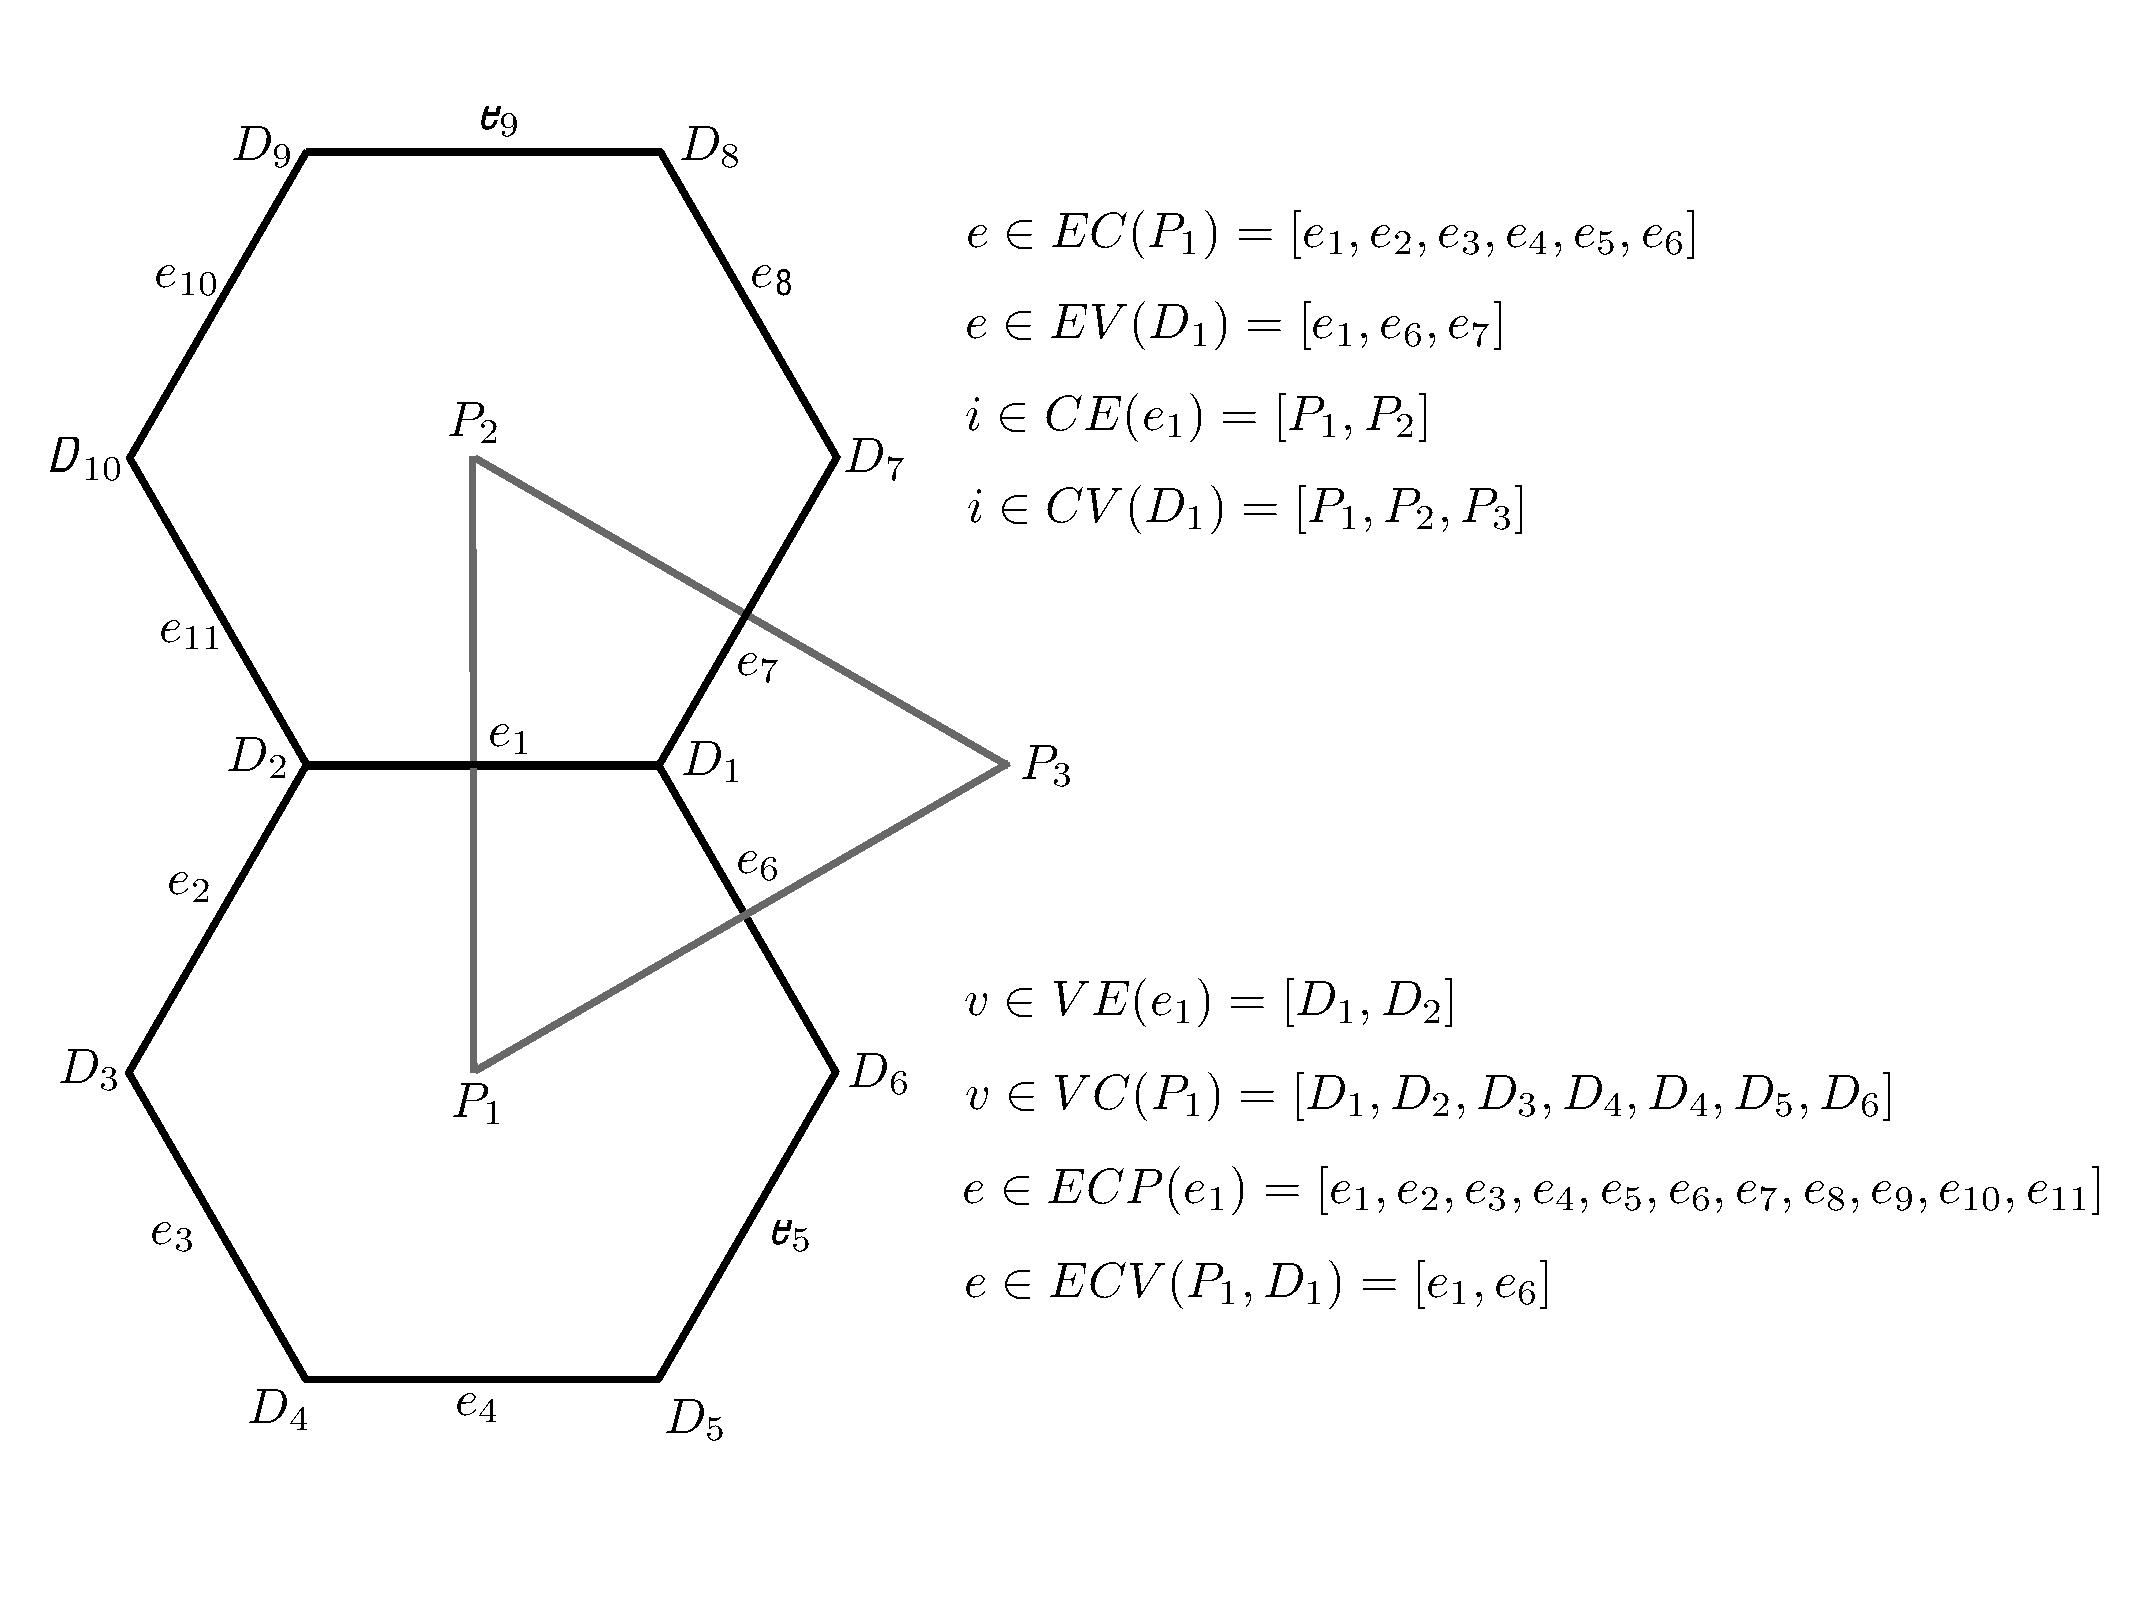
\includegraphics[width=16cm,angle=0]{./shared/figures/gridConnectivity.pdf}\\
  \caption{Definition of element groups used to reference connections in the MPAS grid. Also see Table \ref{table:gridConnectivity}.}
  \label{figure:gridConnectivity}
\end{figure}



\chapter{Configuring Model Input and Output}
\label{chap:mpas_io}

\newlength{\immindent}
\settowidth{\immindent}{{\tt <immutable\_stream }}


\newlength{\mutindent}
\settowidth{\mutindent}{{\tt <stream }}

The reading and writing of model fields in MPAS is handled by user-configurable {\em streams}. 
A stream represents a fixed set of model fields, together with dimensions and attributes, that are
all written or read together to or from the same file or set of files. Each MPAS model core may define
its own set of default streams that it typically uses for reading initial conditions, for writing and reading
restart fields, and for writing additional model history fields. Besides these default streams, users may define
new streams to, e.g., write certain diagnostic fields at a higher temporal frequency than the usual model
history fields.

Streams are defined in XML configuration files that are created at build time for each model core. The name
of this XML file is simply `streams.' suffixed with the name of the core. For example, the streams for
the {\em sw} (shallow-water) core are defined in a file named `streams.sw'. An XML stream
file may further reference other text files that contain lists of the model fields that are read or written in
each of the streams defined in the XML stream file.

Changes to the XML stream configuration file will take effect the next time an MPAS core is run; there is no need
to re-compile after making modifications to the XML files. As described in the next section, it is therefore possible, e.g.,
to change the interval at which a stream is written, the template for the filenames associated with a stream, or the 
set of fields that are written to a stream, without the need to re-compile any code.

Two classes of streams exist in MPAS: {\em immutable} streams and {\em mutable} streams. Immutable streams
are those for which the set of fields that belong to the stream may not be modified at model run-time; however, it is
possible to modify the interval at which the stream is read or written, the filename template describing the files
containing the stream on disk, and several other parameters of the stream. In contrast, all aspects of mutable streams,
including the set of fields that belong to the stream, may be modified at run-time. The motivation for the creation of
two stream classes is the idea that an MPAS core may not function correctly if certain fields are not read in upon 
model start-up or written to restart files, and it is therefore not reasonable for users to modify this set of required fields 
at run-time. An MPAS core developer may choose to implement such streams as immutable streams. Since fields may
not be added to an immutable stream at run-time, new immutable streams may not be defined at run-time, and the only 
type of new stream that may be defined at run-time is the mutable stream type.

\section{XML stream configuration files}
\label{sec:xml_stream_format} 

The XML stream configuration file for an MPAS core always has a parent XML {\em element} named {\tt streams}, within which 
individual streams are defined:

\vspace{12pt}
\noindent {\tt <streams>} \newline
\newline
\hspace*{1cm}... one or more stream definitions ... \newline
\newline
\noindent {\tt </streams>} \newline
\vspace{12pt}

Immutable streams are defined with the {\tt immutable\_stream} element, and mutable streams are defined with the {\tt stream}
element: 

\vspace{12pt}
\noindent {\tt <immutable\_stream name="initial\_conditions"} \newline
\hspace*{\immindent}{\tt type="input"} \newline
\hspace*{\immindent}{\tt filename\_template="init.nc"} \newline
\hspace*{\immindent}{\tt input\_interval="initial\_only"} \newline
\hspace*{\immindent}{\tt />} \newline
\vspace{12pt} \newline
\noindent {\tt <stream name="history"} \newline
\hspace*{\mutindent}{\tt type="output"} \newline
\hspace*{\mutindent}{\tt filename\_template="output.\$Y-\$M-\$D\_\$h.\$m.\$s.nc"} \newline
\hspace*{\mutindent}{\tt output\_interval="6:00:00" >} \newline
\newline
\hspace*{1cm}... model fields belonging to this stream ... \newline
\newline
\noindent {\tt </stream>} \newline
\vspace{12pt}

As shown in the example stream definitions, above, both classes of stream have the following required attributes:

\begin{itemize}
\item {\tt name} --- A unique name used to refer to the stream.
\item {\tt type} --- The type of stream, either {\tt "input"}, {\tt "output"}, {\tt "input;output"}, or {\tt "none"}. A stream may be both an input
and an output stream (i.e., {\tt "input;output"}) if, for example, it is read once at model start-up to provide initial conditions and thereafter written 
periodically to provide model checkpoints. A stream may be defined as neither input nor output (i.e., {\tt "none"}) for the purposes of defining a 
set of fields for inclusion other streams. Note that, for immutable streams, the type attribute may not be changed at run-time.
\item {\tt filename\_template} --- The template for files that exist or will be created by the stream. The filename template may include any of the
following variables, which are expanded based on the simulated time at which files are first created.
\begin{itemize}
\item {\tt \$Y} --- Year
\item {\tt \$M} --- Month
\item {\tt \$D} --- Day of the month
\item {\tt \$d} --- Day of the year
\item {\tt \$h} --- Hour
\item {\tt \$m} --- Minute
\item {\tt \$s} --- Second
\end{itemize}
A filename template may include either a relative or an absolute path, in which case MPAS will attempt to create any directories 
in the path that do not exist, subject to filesystem permissions.
\item {\tt input\_interval} --- For streams that have type {\tt "input"} or {\tt "input;output"}, the interval, beginning at the model initial time,
at which the stream will be read. Possible values include a time interval specification in the format {\tt "YYYY-MM-DD\_hh:mm:ss"}; the value 
{\tt "initial\_only"}, which specifies that the stream is read only once at the model initial time; or the value {\tt "none"}, which specifies that 
the stream is not read during a model run.
\item {\tt output\_interval} --- For streams that have type {\tt "output"} or {\tt "input;output"}, the interval, beginning at the model initial time,
at which the stream will be written. Possible values include a time interval specification in the format {\tt "YYYY-MM-DD\_hh:mm:ss"}; the value 
{\tt "initial\_only"}, which specifies that the stream is written only once at the model initial time; or the value {\tt "none"}, which specifies that 
the stream is not written during a model run.
\end{itemize}

Finally, the set of fields that belong to a mutable stream may be specified with any combination of the following elements. Note that, for 
immutable streams, no fields are specified at run-time in the XML configuration file.

\begin{itemize}
\item {\tt var} --- Associates the specified variable with the stream. The variable may be any of those defined in an MPAS core's Registry.xml file, but may
not include individual constituent arrays from a var\_array.
\item {\tt var\_array} --- Associates all constituent variables in a var\_array, defined in an MPAS core's Registry.xml file, with the stream.
\item {\tt var\_struct} --- Associates all variables in a var\_struct, defined in an MPAS core's Registry.xml file, with the stream.
\item {\tt stream} --- Associates all explicitly associated fields in the specified stream with the stream; streams are not recursively included.
\item {\tt file} --- Associates all variables listed in the specified text file, with one field per line, with the stream.
\end{itemize}

\section{Optional stream attributes}
\label{sec:optional_stream_atts} 

Besides the required attributes described in the preceding section, several additional, optional attributes may be added to
the definition of a stream.

\begin{itemize}
\item {\tt filename\_interval} --- The interval between the timestamps used in the construction of the names of files associated with
a stream. Possible values include a time interval specification in the format {\tt "YYYY-MM-DD\_hh:mm:ss"}; the value {\tt "none"}, indicating
that only one file containing all times is associated with the stream; the value {\tt "input\_interval"} that, for input type streams, indicates that
each time to be read from the stream will come from a unique file; or the value {\tt "output\_interval"} that, for output type streams, indicates 
that each time to be written to the stream will go to a unique file whose name is based on the timestamp of the data being written. The default
value is {\tt "input\_interval"} for input type streams and {\tt "output\_interval"} for output type streams. For streams of type {\tt "input;output"}, the
default filename interval is {\tt "input\_interval"} if the input interval is an interval (i.e., not {\tt "initial\_only"}), or {\tt "output\_interval"} otherwise. 
Refer to Section \ref{sec:filename_interval_example}
for an example of the use of the filename\_interval attribute.
\item {\tt reference\_time} --- A time that is an integral number of filename intervals from the timestamp of any file associated with the stream.
The default value is the start time of the model simulation. Refer to Section \ref{sec:reference_time_example} for an example of 
the use of the reference\_time attribute.
\item {\tt clobber\_mode} --- Specifies how a stream should handle attempts to write to a file that already exists. Possible values
for the mode include:
\begin{itemize}
\item {\tt "overwrite"} --- The stream is allowed to overwrite records in existing files and to append new records 
to existing files; records not explicitly written to are left untouched.
\item {\tt "truncate"} or {\tt "replace\_files"} --- The stream is allowed to overwrite existing files, which are first truncated 
to remove any existing records; this is equivalent to replacing any existing files with newly created files of the same name.
\item {\tt "append"} --- The stream is only allowed to append new records to existing files; existing records may not be overwritten.
\item {\tt "never\_modify"} --- The stream is not allowed to modify existing files in any way.
\end{itemize}
The default clobber mode for streams is {\tt "never\_modify"}. Refer to Section \ref{sec:append_example} for an example of the use of
the clobber\_mode attribute.
\item {\tt precision} --- The precision with which real-valued fields will be written or read in a stream. Possible values include 
{\tt "single"} for 4-byte real values, {\tt "double"} for 8-byte real values, or {\tt "native"}, which specifies that real-valued fields
will be written or read in whatever precision the MPAS core was compiled. The default value is {\tt "native"}. Refer to Section \ref{sec:filename_interval_example}
for an example of the use of the precision attribute.
\item {\tt packages} --- A list of packages attached to the stream. A stream will be active (i.e., read or written) only if at least one of 
the packages attached to it is active, or if no packages at all are attached. Package names are provided as a semi-colon-separated
list. Note that packages may only be defined in an MPAS core's Registry.xml file at build time. By default, no packages are attached
to a stream.
\item {\tt io\_type} --- The underlying library and file format that will be used to read or write a stream. Possible values include:
\begin{itemize}
\item{\tt "pnetcdf"} --- Read/write the stream with classic large-file NetCDF files (CDF-2) using the ANL Parallel-NetCDF library.
\item{\tt "pnetcdf,cdf5"} --- Read/write the stream with large-variable files (CDF-5) using the ANL Parallel-NetCDF library. 
\item{\tt "netcdf"} --- Read/write the stream with classic large-file NetCDF files (CDF-2) using the Unidata serial NetCDF library.
\item{\tt "netcdf4"} --- Read/write the stream with HDF-5 files using the Unidata parallel NetCDF-4 library.
\end{itemize}
Note that the PIO library must have been built with support for the selected {\tt io\_type}. By default, all input and output streams are
read and written using the {\tt "pnetcdf"} option.
\end{itemize}

\section{Stream definition examples}
\label{sec:stream_example} 

This section provides several example streams that make use of the optional stream attributes described in Section \ref{sec:optional_stream_atts}.
All examples are of output streams, since it is more likely that a user will need to write additional fields than to read additional fields, which a model would need to be aware of; however, the concepts that are illustrated here translate directly to input streams as well.

\subsection{Example: a single-precision output stream with one month of data per file}
\label{sec:filename_interval_example}

In this example, the optional attribute specification {\tt filename\_interval="01-00\_00:00:00"} is added to force a new
output file to be created for the stream every month. Note that the general format for time interval specifications is {\tt YYYY-MM-DD\_hh:mm:ss},
where any leading terms can be omitted; in this case, the year part of the interval is omitted. To reduce the file size, the specification
{\tt precision="single"} is also added to force real-valued fields to be written as 4-byte floating-point values, rather than the default of 8 bytes.

\vspace{12pt}
\noindent {\tt <stream name="diagnostics"} \newline
\hspace*{\mutindent}{\tt type="output"} \newline
\hspace*{\mutindent}{\tt filename\_template="diagnostics.\$Y-\$M.nc"} \newline
\hspace*{\mutindent}{\tt filename\_interval="01-00\_00:00:00"} \newline
\hspace*{\mutindent}{\tt precision="single"} \newline
\hspace*{\mutindent}{\tt output\_interval="6:00:00" >} \newline
\newline
\hspace*{1cm}{\tt <var name="u10"/>} \newline
\hspace*{1cm}{\tt <var name="v10"/>} \newline
\hspace*{1cm}{\tt <var name="t2"/>} \newline
\hspace*{1cm}{\tt <var name="q2"/>} \newline
\newline
\noindent {\tt </stream>} \newline
\vspace{12pt}

The only fields that will be written to this stream are the hypothetical 10-m diagnosed wind components, the 2-m temperature, 
and the 2-m specific humidity variables. Also, note that the filename template only includes the year and month from the model 
valid time; this can be problematic when the simulation starts in the middle of a month, and a solution for this problem 
is illustrated in the example of Section \ref{sec:reference_time_example}.

\subsection{Example: appending records to existing output files}
\label{sec:append_example}

By default, streams will never modify existing files whose filenames match the name of a file that would otherwise be written
during the course of a simulation. However, when restarting a simulation that is expected to add more records to existing output 
files, it can be useful to instruct the MPAS I/O system to append these records, thereby modifying existing files. This may be 
accomplished with the {\tt clobber\_mode} attribute.

\vspace{12pt}
\noindent {\tt <stream name="diagnostics"} \newline
\hspace*{\mutindent}{\tt type="output"} \newline
\hspace*{\mutindent}{\tt filename\_template="diagnostics.\$Y-\$M.nc"} \newline
\hspace*{\mutindent}{\tt filename\_interval="01-00\_00:00:00"} \newline
\hspace*{\mutindent}{\tt precision="single"} \newline
\hspace*{\mutindent}{\tt clobber\_mode="append"} \newline
\hspace*{\mutindent}{\tt output\_interval="6:00:00" >} \newline
\newline
\hspace*{1cm}{\tt <var name="u10"/>} \newline
\hspace*{1cm}{\tt <var name="v10"/>} \newline
\hspace*{1cm}{\tt <var name="t2"/>} \newline
\hspace*{1cm}{\tt <var name="q2"/>} \newline
\newline
\noindent {\tt </stream>} \newline
\vspace{12pt}

In general, if MPAS were to attempt to write a record at a time that already existed in an output file, a clobber\_mode 
of `append' would not permit the write to take place, since this would modify existing data; in `append' mode, only new
records may be added. However, due to a peculiarity in the implementation of the `append' clobber mode, it may be 
possible for an output file to contain duplicate times. This can happen when the first record that is appended to 
an existing file has a timestamp not matching any in the file, after which, any record that is written --- regardless of 
whether its timestamp matches one already in the file --- will be appended to the end of the file. This situation may arise, 
for example, when restarting a model simulation with a shorter {\tt output\_interval} than was used in the original model simulation 
with an MPAS core that does not write the first output time for restart runs.

\subsection{Example: referencing filename intervals to a time other than the start time}
\label{sec:reference_time_example}

The example stream of the previous sections creates a new file each month during the simulation, and the filenames
contain only the year and month of the timestamp when the file was created. If a simulation begins at 00 UTC on the
first day of a month, then each file in the diagnostic stream will contain only output times that fall within the month
in the filename. However, if a simulation were to begin in the middle of a month --- for example, the month of June, 2014 --- 
the first diagnostics output file would have a filename of `diagnostics.2014-06.nc', but rather than containing only output
fields valid in June, it would contain all fields written between the middle of June and the middle of July, at which point
one month of simulation would have elapsed, and a new output file, `diagnostics.2014-07.nc', would be created.

In order to ensure that the file `diagnostics.2014-06.nc' contained only data from June 2014, the {\tt reference\_time}
attribute may be added such that the day, hour, minute, and second in the date and time represent the first day of the month
at 00 UTC. In this example, the year and month of the reference time are not important, since the purpose of the reference time
here is to describe to MPAS that the monthly filename interval begins (i.e., is referenced to) the first day of the month.

\vspace{12pt}
\noindent {\tt <stream name="diagnostics"} \newline
\hspace*{\mutindent}{\tt type="output"} \newline
\hspace*{\mutindent}{\tt filename\_template="diagnostics.\$Y-\$M.nc"} \newline
\hspace*{\mutindent}{\tt filename\_interval="01-00\_00:00:00"} \newline
\hspace*{\mutindent}{\tt reference\_time="2014-01-01\_00:00:00"} \newline
\hspace*{\mutindent}{\tt precision="single"} \newline
\hspace*{\mutindent}{\tt clobber\_mode="append"} \newline
\hspace*{\mutindent}{\tt output\_interval="6:00:00" >} \newline
\newline
\hspace*{1cm}{\tt <var name="u10"/>} \newline
\hspace*{1cm}{\tt <var name="v10"/>} \newline
\hspace*{1cm}{\tt <var name="t2"/>} \newline
\hspace*{1cm}{\tt <var name="q2"/>} \newline
\newline
\noindent {\tt </stream>} \newline
\vspace{12pt}

In general, the components of a timestamp, {\tt YYYY-MM-DD\_hh:mm:ss}, that are less significant than (i.e., to the right of) 
those contained in a filename template are important in a reference\_time. For example, with a {\tt filename\_template} that contained
only the year, the month component of the {\tt reference\_time} would become important to identify the month of the year on which
the yearly basis for filenames would begin.



% Grid generation is not included in MPAS release 1.0:
%\appendix{Generating meshes}
\label{chap:mpas_grid_generation}

This chapter describes the steps used to create the  spherical centroidal Voronoi tessellation (SCVT) meshes and mesh-decomposition files used by MPAS models.
Since it can take considerable time (often several days or more) to generate a mesh as described in \S \ref{sec:global_scvt}, it is recommended to obtain 
and use existing SCVT meshes from \url{http://www.mmm.ucar.edu/people/duda/mpas/} whenever possible; these meshes can be quickly
modified to shift or rotate the refinement regions over the geographic areas of interest using the utility program described in \S \ref{sec:grid_rotate}.

\section{Density functions}

In all MPAS models, the horizontal meshes are SCVTs with a C-grid staggering of
velocities. As their name suggests, SCVTs are Voronoi tessellations defined on the surface of a sphere, and in which the generating 
point for each Voronoi region is also the mass centroid of that region with respect to some {\em density function}. An overview of
the application of SCVTs to multi-resolution climate modeling is given in Ringler et al. (2008)
\footnote{Ringler, T., L. Ju and M. Gunzburger, 2008, A multiresolution method for climate system modeling: application of spherical centroidal Voronoi tessellations, {\em Ocean Dynamics}, 58 (5-6), 475-498. doi:10.1007/s10236-008-0157-2.}.

For the purposes of generating SCVTs, the central concern lies with the density function, $\rho$, which is a user-defined
function relating the relative resolutions in different regions of the mesh. Specifically, for two generating points of the 
SCVT, ${\bf x}_i$ and ${\bf x}_j$,
\[
{h_i \over h_j} \approx \left({\rho({\bf x}_j) \over \rho({\bf x}_i)} \right)^{1 \over 4},
\]
where $h_i$ and $h_j$ are the diameters of the Voronoi cells associated with ${\bf x}_i$ and ${\bf x}_j$, respectively.

In the mesh generation program global\_scvt, described in the next section, the density function is defined programatically in the Fortran function
{\tt density\_for\_point()}, which returns the value of the density function, $\rho({\bf x})$, given a location on the sphere, ${\bf x}$.
   
\section{The global\_scvt program}
\label{sec:global_scvt}

\subsection{Compilation}
                                                                                             
As a first step toward building the global\_scvt code, the environment variable                     
{\tt NETCDF} must be set to the root of the netCDF installation. Unlike with the MPAS model, separate make targets are not
defined for each compiler set, and it will generally be necessary to edit the top-level Makefile to set the compiler and compiler flags                 
that will be used to build global\_scvt; however, there are commented-out sections in the Makefile for using either of the ifort, pgf90, or gfortran compilers that may be uncommented or used as a starting point for other compilers. Also, if the netCDF installation has a separate Fortran interface library, {\tt -lnetcdff} will need to be added before {\tt -lnetcdf} in the Makefile. The global\_scvt program is parallelized with OpenMP, so if compiler support is available, OpenMP compiler flags may be added
in the Makefile as well.                      

Before compiling the global\_scvt program, a density function should first be defined in the function {\tt density\_for\_point()} in {\tt src/module\_scvt.F}. The default density function is a uniform density function that returns a value of 1.0 for all locations
on the sphere, and commented code in {\tt density\_for\_point()} may be uncommented to achieve an area of circular refinement. {\em Note that, although $\rho({\bf x})$ could in principle take on any non-negative value, the code to scale eddy viscosities by the mesh resolution in the MPAS model assumes that $\rho({\bf x}) \in (0,1]$, so care should be taken when designing a new density function: a value of 1.0 should correspond to the highest-resolution regions(s) in the mesh.}                                      
                                                                                                
After editing the Makefile and defining the desired density function, running `make' should create the grid\_gen executable 
in the top-level directory. A second program, grid\_ref, may also be created, but this program is not needed by the current version 
of the global\_scvt program.

\subsection{Running}

As will be described in Section \ref{sec:grid_gen_efficiency}, a typical mesh is generated using multiple refinement steps. Within each of these steps, an SCVT with a fixed
number of generating points is converged before the SCVT is refined, giving a larger number of generating points to begin the next step. In this section, the process of converging an SCVT within a single step is described.

Two files are needed in order to run the grid\_gen program: an initial generating point file, {\tt locs.dat}, and a                        
namelist file, {\tt namelist.input}. The {\tt locs.dat} file contains a list of the Cartesian coordinates (assuming a unit-radius sphere
centered at the origin) of each of the beginning generating points, and the {\tt namelist.input} file specifies the number of generating points to be read from the {\tt locs.dat} file, the number of iterations to run, and the convergence criteria; a complete list of namelist variables is provided in the table below.

\vspace{12pt}
\begin{longtable}{|p{1.25in} |p{4.5in}|}
\hline
np & the number of points to read from the {\tt locs.dat} file \\ \hline
locs\_as\_xyz & whether the initial generating points in {\tt locs.dat} are given in Cartesian space ({\tt .true.}) or latitude-longitude space ({\tt .false.}) \\ \hline
n\_scvt\_iterations & the maximum number of Lloyd iterations to perform \\ \hline
eps & the convergence criterion, specifying the maximum permissible average movement of a generating point during an iteration \\ \hline
l2\_conv & whether to stop iterating if the convergence criterion is met \\ \hline
inf\_conv & currently the same meaning as l2\_conv \\ \hline
min\_dx & the targeted minimum grid distance in the mesh, on which an estimate for the number of generating points will be based; see Section \ref{sec:estimating_np} \\ \hline
\end{longtable}
\vspace{12pt}

\noindent A convergence criterion of $1\times10^{-10}$ should be sufficient, and in                     
practice, many thousands of iterations are needed to reach this tolerance.

If grid\_gen was compiled with OpenMP support, the environment variable {\tt OMP\_NUM\_THREADS} can be set to the 
number of threads that will be used by the program. Then, grid\_gen can be run with no command-line arguments:

\vspace{12pt}
{\tt > ./grid\_gen}
\vspace{12pt}
                                                                                         
                                                                                                
When grid\_gen finishes --- either because the convergence criterion has been met, or the
maximum number of iterations have been performed ---  several output files should be created: 

\begin{itemize}
\item {\tt scvt\_initial.ps} --- a plot of the mesh at the start of iterations,
\item {\tt scvt\_final.ps} --- a plot of the mesh after iterations,
\item {\tt grid.nc} --- the actual MPAS mesh file, which can be used with the initialization core to create an MPAS input file,
\item {\tt graph.info} --- information describing the cell connectivity graph of the mesh, to be used with a graph partitioner as described in Section \ref{sec:metis}, and
\item {\tt locs.dat.out} --- a list of the final generating points appended with a set of $3 np - 6$ refinement points. 
\end{itemize}

If the tolerance specified in the {\tt namelist.input} file was met, the SCVT mesh should be sufficiently converged, and the resulting {\tt grid.nc}
file can be used with the initialization program to create an initial condition file for MPAS; alternatively, the full set of $4 np - 6$ refinement points in 
the {\tt locs.dat.out} file can be used as input to the grid\_gen program to create another SCVT with approximately twice the resolution. If, however, the specified tolerance was not met, the {\tt locs.dat.out} file may be copied to {\tt locs.dat}, and further iteration may be performed on the SCVT.

To create a plot of the mesh with coastlines, which can be helpful when locating or sizing refinement regions, the {\tt mesh.ncl} script may be used to plot the mesh directly from                 
the {\tt grid.nc} file.                                                                          

\subsection{Estimating the required number of generating points}
\label{sec:estimating_np}

Setting the {\tt min\_dx} variable in the {\tt namelist.input} file to the targeted minimum grid distance in the mesh and running the grid\_gen program will cause the program to print out an estimate for the number of generating points that will be required to achieve that minimum grid distance with the density function provided in {\tt density\_for\_point()}.

\subsection{Efficiency concerns}
\label{sec:grid_gen_efficiency}

Although one could, given an estimate for the number of generating points needed to achieve the required absolute resolutions in the mesh,
create a {\tt locs.dat} file with that number of randomly chosen points on the unit sphere, and, using that {\tt locs.dat} file, converge a final SCVT, 
experience indicates that a stepwise approach can significantly reduce the required wallclock time.                   

   
\section{The grid\_rotate program} 
\label{sec:grid_rotate} 

The purpose of the grid\_rotate program is simply to rotate an MPAS mesh file, moving a refinement region from one geographic location to another, so that the mesh can be re-used for different applications. This utility was developed out of the need to save computational resources, since generating an SCVT --- particularly one with a large number of generating points or a high degree of refinement --- can take considerable time.

To build the grid\_rotate program, the Makefile should first be edited to set the Fortran compiler to be used; if the netCDF installation pointed to by the {\tt NETCDF} environment variable was build with a separate Fortran interface library, it will also be necessary to add {\tt -lnetcdff} just before {\tt -lnetcdf} in the Makefile. After editing the Makefile, running `make' should result in a grid\_rotate executable file.

Besides the MPAS grid file to be rotated, grid\_rotate requires a namelist file, {\tt namelist.input}, which specifies the rotation to be applied to the mesh. The namelist variables are summarized in the table below
   
\vspace{12pt}
\begin{longtable}{|p{3.25in} |p{2.5in}|}
\hline
config\_original\_latitude\_degrees & original latitude of any point on the sphere \\ \hline
config\_original\_longitude\_degrees & original longitude of any point on the sphere \\ \hline
config\_new\_latitude\_degrees &  latitude to which the original point should be shifted \\ \hline
config\_new\_longitude\_degrees &  longitude to which the original point should be shifted \\ \hline
config\_birdseye\_rotation\_counter\_clockwise\_degrees & rotation about a vector from the sphere center through the original point \\ \hline
\end{longtable}
\vspace{12pt}

\noindent Essentially, one chooses any point on the sphere, decides where that point should be shifted to,
and specifies any change to the orientation (i.e., rotation) of the mesh about that point. 

Having set the rotation parameters in the {\tt namelist.input} file, the grid\_rotate program should be run with two command-line options
specifying the original grid file name and the name of the rotated grid file to be produced, e.g.,

\vspace{12pt}
{\tt > grid\_rotate grid.nc grid\_SE\_Asia\_refinement.nc}
\vspace{12pt}

The original grid file will not be altered, and a new, rotated grid file will be created. The NCL script {\tt mesh.ncl} may be used to plot either of the original or rotated grid files after suitable setting the name of the grid file in the script.
   
   
\section{Graph partitioning with METIS} 
\label{sec:metis}

{\color{red} THIS SECTION WAS COPIED TO mpas_build_instructions.tex  FOR RELEASE 1.0. WHEN GRID GENERATION IS INCLUDED, DELETE THE METIS SECTION FROM mpas_build_instructions.tex}.

Before MPAS can be run in parallel, a mesh decomposition file with an appropriate number of 
partitions (equal to the number of MPI tasks that will be used) is required in the run directory.  A limited number of mesh decomposition files ({\tt graph.info.part.*}) are provided with each test case (see Test Cases Chapter).  In order to create new mesh decomposition files for your desired number of partitions, begin with the {\tt graph.info} file created by the grid\_gen program or available with your test case, and partition with METIS software (\url{http://glaros.dtc.umn.edu/gkhome/views/metis}). The serial graph partitioning program, METIS (rather than ParMETIS or hMETIS) should be sufficient for quickly partitioning any SCVT produced by the grid\_gen mesh generator.

After installing METIS, a {\tt graph.info} file may be partitioned into $N$ partitions by running

\vspace{12pt}
{\tt > gpmetis graph.info} $N$
\vspace{12pt}

\noindent The resulting file, {\tt graph.info.part.}$N$, can then be copied into the MPAS run directory
before running the model with $N$ MPI tasks.


%--------------------------------------------------------------------------------------------
% Plotting model output
%--------------------------------------------------------------------------------------------

\chapter{Visualization}
\label{chap:mpas_visualization}

This chapter discusses visualization tools that may be used by all cores.  For instructions on additional visualization tools for this core, see Chapter \ref{chap:\core_visualization}.

\section{ParaView}

ParaView may be used to visualize MPAS initialization, output, and restart files.  It includes a reader that was specifically designed to read MPAS NetCDF files, including Cartesian and spherical domains.  At this time, only cell-centered quantities may be plotted with ParaView.  Variables located at edges and vertices must be interpolated to cell centers for visualization.

ParaView is freely available for download at \url{http://www.paraview.org}.  Binary installations are available for Windows, Mac, and Linux, as well as source code files and tutorials.  From the ParaView website:
\begin{quotation}
ParaView is an open-source, multi-platform data analysis and visualization application. ParaView users can quickly build visualizations to analyze their data using qualitative and quantitative techniques. The data exploration can be done interactively in 3D or programmatically using ParaView's batch processing capabilities.  ParaView was developed to analyze extremely large datasets using distributed memory computing resources. It can be run on supercomputers to analyze datasets of terascale as well as on laptops for smaller data.
\end{quotation}

To visualize an MPAS cell-centered variable in ParaView, open the file and choose {\tt MPAS NetCDF (Unstructured)} as the file format.  In the lower left Object Inspector panel, choose your variables of interest (Figure \ref{fig:ParaviewExample}).  For large data sets, loading fewer variables will result in less wait time.  Options are available for latitude-longitude projections, vertical level, etc.  Click the 'Apply' button to load the data set.  In the toolbars at the top, choose the variable to plot from the pull-down menu, and 'Surface' for the type of visualization.  The color bar button displays a color bar, and the color scale editor button allows the user to manually change the color bar type and extents.  The Filters menu provides computational tools for interactive data manipulation.  Movies, in avi format or as individual frames, may be conveniently created with the {\tt Save Animation} tool in the File menu.


\begin{figure}[htb]
\begin{center}
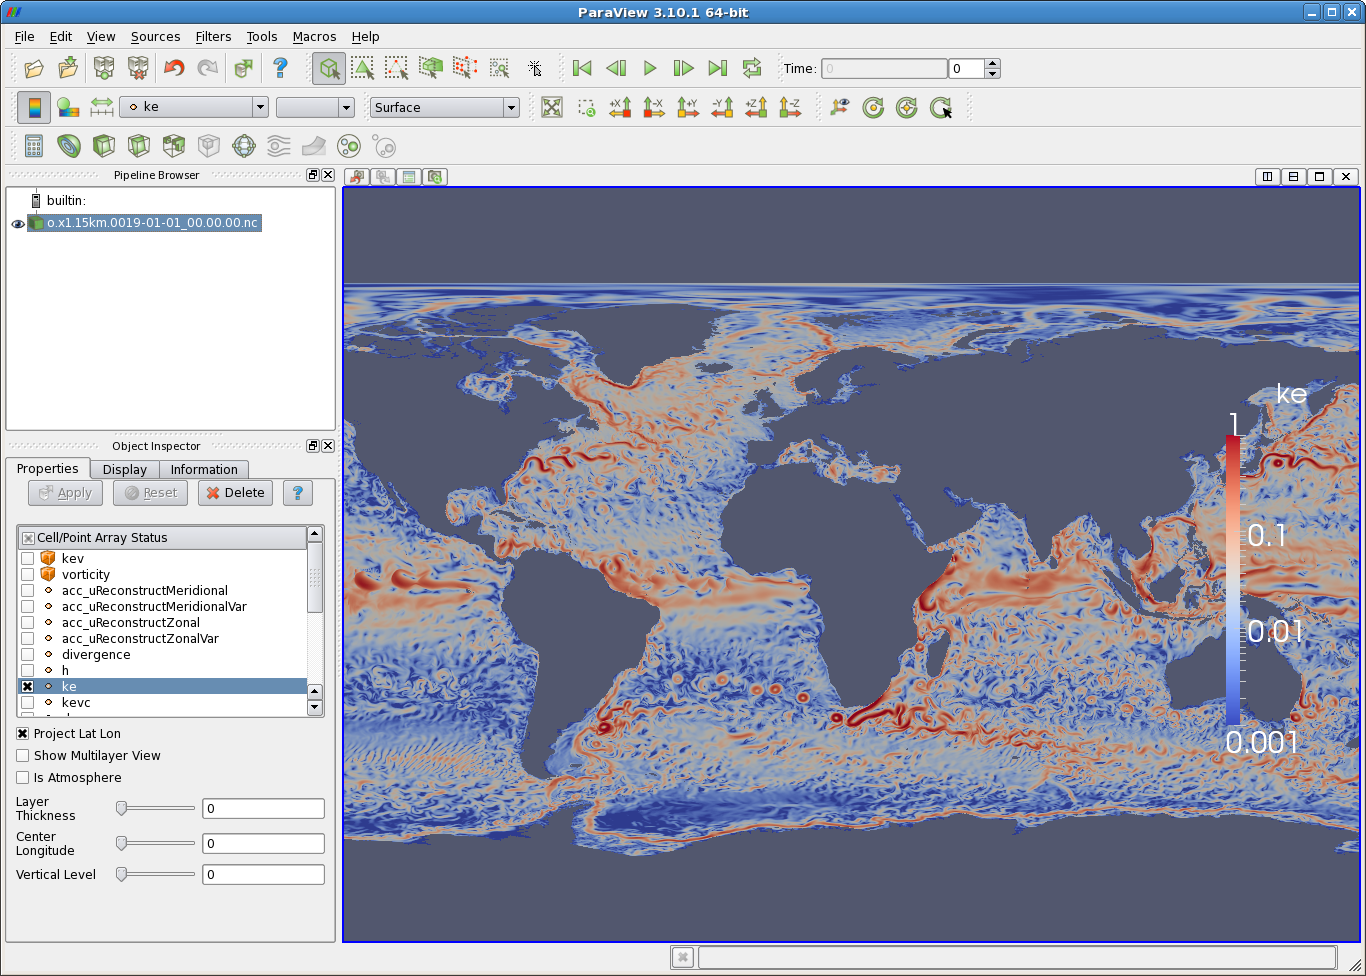
\includegraphics[width=6.5in]{shared/figures/ParaviewExample.png}
\caption{Example of ParaView to view an MPAS NetCDF file.}
\label{fig:ParaviewExample}
\end{center}
\end{figure}


\part{MPAS-Seaice}

% Grid generation is not included in MPAS release 1.0.
% In a future release, describe here ocean-specific grid
% generation, currently the basin.F program.
%\appendix{Generating meshes}
\label{chap:mpas_grid_generation}

This chapter describes the steps used to create the  spherical centroidal Voronoi tessellation (SCVT) meshes and mesh-decomposition files used by MPAS models.
Since it can take considerable time (often several days or more) to generate a mesh as described in \S \ref{sec:global_scvt}, it is recommended to obtain 
and use existing SCVT meshes from \url{http://www.mmm.ucar.edu/people/duda/mpas/} whenever possible; these meshes can be quickly
modified to shift or rotate the refinement regions over the geographic areas of interest using the utility program described in \S \ref{sec:grid_rotate}.

\section{Density functions}

In all MPAS models, the horizontal meshes are SCVTs with a C-grid staggering of
velocities. As their name suggests, SCVTs are Voronoi tessellations defined on the surface of a sphere, and in which the generating 
point for each Voronoi region is also the mass centroid of that region with respect to some {\em density function}. An overview of
the application of SCVTs to multi-resolution climate modeling is given in Ringler et al. (2008)
\footnote{Ringler, T., L. Ju and M. Gunzburger, 2008, A multiresolution method for climate system modeling: application of spherical centroidal Voronoi tessellations, {\em Ocean Dynamics}, 58 (5-6), 475-498. doi:10.1007/s10236-008-0157-2.}.

For the purposes of generating SCVTs, the central concern lies with the density function, $\rho$, which is a user-defined
function relating the relative resolutions in different regions of the mesh. Specifically, for two generating points of the 
SCVT, ${\bf x}_i$ and ${\bf x}_j$,
\[
{h_i \over h_j} \approx \left({\rho({\bf x}_j) \over \rho({\bf x}_i)} \right)^{1 \over 4},
\]
where $h_i$ and $h_j$ are the diameters of the Voronoi cells associated with ${\bf x}_i$ and ${\bf x}_j$, respectively.

In the mesh generation program global\_scvt, described in the next section, the density function is defined programatically in the Fortran function
{\tt density\_for\_point()}, which returns the value of the density function, $\rho({\bf x})$, given a location on the sphere, ${\bf x}$.
   
\section{The global\_scvt program}
\label{sec:global_scvt}

\subsection{Compilation}
                                                                                             
As a first step toward building the global\_scvt code, the environment variable                     
{\tt NETCDF} must be set to the root of the netCDF installation. Unlike with the MPAS model, separate make targets are not
defined for each compiler set, and it will generally be necessary to edit the top-level Makefile to set the compiler and compiler flags                 
that will be used to build global\_scvt; however, there are commented-out sections in the Makefile for using either of the ifort, pgf90, or gfortran compilers that may be uncommented or used as a starting point for other compilers. Also, if the netCDF installation has a separate Fortran interface library, {\tt -lnetcdff} will need to be added before {\tt -lnetcdf} in the Makefile. The global\_scvt program is parallelized with OpenMP, so if compiler support is available, OpenMP compiler flags may be added
in the Makefile as well.                      

Before compiling the global\_scvt program, a density function should first be defined in the function {\tt density\_for\_point()} in {\tt src/module\_scvt.F}. The default density function is a uniform density function that returns a value of 1.0 for all locations
on the sphere, and commented code in {\tt density\_for\_point()} may be uncommented to achieve an area of circular refinement. {\em Note that, although $\rho({\bf x})$ could in principle take on any non-negative value, the code to scale eddy viscosities by the mesh resolution in the MPAS model assumes that $\rho({\bf x}) \in (0,1]$, so care should be taken when designing a new density function: a value of 1.0 should correspond to the highest-resolution regions(s) in the mesh.}                                      
                                                                                                
After editing the Makefile and defining the desired density function, running `make' should create the grid\_gen executable 
in the top-level directory. A second program, grid\_ref, may also be created, but this program is not needed by the current version 
of the global\_scvt program.

\subsection{Running}

As will be described in Section \ref{sec:grid_gen_efficiency}, a typical mesh is generated using multiple refinement steps. Within each of these steps, an SCVT with a fixed
number of generating points is converged before the SCVT is refined, giving a larger number of generating points to begin the next step. In this section, the process of converging an SCVT within a single step is described.

Two files are needed in order to run the grid\_gen program: an initial generating point file, {\tt locs.dat}, and a                        
namelist file, {\tt namelist.input}. The {\tt locs.dat} file contains a list of the Cartesian coordinates (assuming a unit-radius sphere
centered at the origin) of each of the beginning generating points, and the {\tt namelist.input} file specifies the number of generating points to be read from the {\tt locs.dat} file, the number of iterations to run, and the convergence criteria; a complete list of namelist variables is provided in the table below.

\vspace{12pt}
\begin{longtable}{|p{1.25in} |p{4.5in}|}
\hline
np & the number of points to read from the {\tt locs.dat} file \\ \hline
locs\_as\_xyz & whether the initial generating points in {\tt locs.dat} are given in Cartesian space ({\tt .true.}) or latitude-longitude space ({\tt .false.}) \\ \hline
n\_scvt\_iterations & the maximum number of Lloyd iterations to perform \\ \hline
eps & the convergence criterion, specifying the maximum permissible average movement of a generating point during an iteration \\ \hline
l2\_conv & whether to stop iterating if the convergence criterion is met \\ \hline
inf\_conv & currently the same meaning as l2\_conv \\ \hline
min\_dx & the targeted minimum grid distance in the mesh, on which an estimate for the number of generating points will be based; see Section \ref{sec:estimating_np} \\ \hline
\end{longtable}
\vspace{12pt}

\noindent A convergence criterion of $1\times10^{-10}$ should be sufficient, and in                     
practice, many thousands of iterations are needed to reach this tolerance.

If grid\_gen was compiled with OpenMP support, the environment variable {\tt OMP\_NUM\_THREADS} can be set to the 
number of threads that will be used by the program. Then, grid\_gen can be run with no command-line arguments:

\vspace{12pt}
{\tt > ./grid\_gen}
\vspace{12pt}
                                                                                         
                                                                                                
When grid\_gen finishes --- either because the convergence criterion has been met, or the
maximum number of iterations have been performed ---  several output files should be created: 

\begin{itemize}
\item {\tt scvt\_initial.ps} --- a plot of the mesh at the start of iterations,
\item {\tt scvt\_final.ps} --- a plot of the mesh after iterations,
\item {\tt grid.nc} --- the actual MPAS mesh file, which can be used with the initialization core to create an MPAS input file,
\item {\tt graph.info} --- information describing the cell connectivity graph of the mesh, to be used with a graph partitioner as described in Section \ref{sec:metis}, and
\item {\tt locs.dat.out} --- a list of the final generating points appended with a set of $3 np - 6$ refinement points. 
\end{itemize}

If the tolerance specified in the {\tt namelist.input} file was met, the SCVT mesh should be sufficiently converged, and the resulting {\tt grid.nc}
file can be used with the initialization program to create an initial condition file for MPAS; alternatively, the full set of $4 np - 6$ refinement points in 
the {\tt locs.dat.out} file can be used as input to the grid\_gen program to create another SCVT with approximately twice the resolution. If, however, the specified tolerance was not met, the {\tt locs.dat.out} file may be copied to {\tt locs.dat}, and further iteration may be performed on the SCVT.

To create a plot of the mesh with coastlines, which can be helpful when locating or sizing refinement regions, the {\tt mesh.ncl} script may be used to plot the mesh directly from                 
the {\tt grid.nc} file.                                                                          

\subsection{Estimating the required number of generating points}
\label{sec:estimating_np}

Setting the {\tt min\_dx} variable in the {\tt namelist.input} file to the targeted minimum grid distance in the mesh and running the grid\_gen program will cause the program to print out an estimate for the number of generating points that will be required to achieve that minimum grid distance with the density function provided in {\tt density\_for\_point()}.

\subsection{Efficiency concerns}
\label{sec:grid_gen_efficiency}

Although one could, given an estimate for the number of generating points needed to achieve the required absolute resolutions in the mesh,
create a {\tt locs.dat} file with that number of randomly chosen points on the unit sphere, and, using that {\tt locs.dat} file, converge a final SCVT, 
experience indicates that a stepwise approach can significantly reduce the required wallclock time.                   

   
\section{The grid\_rotate program} 
\label{sec:grid_rotate} 

The purpose of the grid\_rotate program is simply to rotate an MPAS mesh file, moving a refinement region from one geographic location to another, so that the mesh can be re-used for different applications. This utility was developed out of the need to save computational resources, since generating an SCVT --- particularly one with a large number of generating points or a high degree of refinement --- can take considerable time.

To build the grid\_rotate program, the Makefile should first be edited to set the Fortran compiler to be used; if the netCDF installation pointed to by the {\tt NETCDF} environment variable was build with a separate Fortran interface library, it will also be necessary to add {\tt -lnetcdff} just before {\tt -lnetcdf} in the Makefile. After editing the Makefile, running `make' should result in a grid\_rotate executable file.

Besides the MPAS grid file to be rotated, grid\_rotate requires a namelist file, {\tt namelist.input}, which specifies the rotation to be applied to the mesh. The namelist variables are summarized in the table below
   
\vspace{12pt}
\begin{longtable}{|p{3.25in} |p{2.5in}|}
\hline
config\_original\_latitude\_degrees & original latitude of any point on the sphere \\ \hline
config\_original\_longitude\_degrees & original longitude of any point on the sphere \\ \hline
config\_new\_latitude\_degrees &  latitude to which the original point should be shifted \\ \hline
config\_new\_longitude\_degrees &  longitude to which the original point should be shifted \\ \hline
config\_birdseye\_rotation\_counter\_clockwise\_degrees & rotation about a vector from the sphere center through the original point \\ \hline
\end{longtable}
\vspace{12pt}

\noindent Essentially, one chooses any point on the sphere, decides where that point should be shifted to,
and specifies any change to the orientation (i.e., rotation) of the mesh about that point. 

Having set the rotation parameters in the {\tt namelist.input} file, the grid\_rotate program should be run with two command-line options
specifying the original grid file name and the name of the rotated grid file to be produced, e.g.,

\vspace{12pt}
{\tt > grid\_rotate grid.nc grid\_SE\_Asia\_refinement.nc}
\vspace{12pt}

The original grid file will not be altered, and a new, rotated grid file will be created. The NCL script {\tt mesh.ncl} may be used to plot either of the original or rotated grid files after suitable setting the name of the grid file in the script.
   
   
\section{Graph partitioning with METIS} 
\label{sec:metis}

{\color{red} THIS SECTION WAS COPIED TO mpas_build_instructions.tex  FOR RELEASE 1.0. WHEN GRID GENERATION IS INCLUDED, DELETE THE METIS SECTION FROM mpas_build_instructions.tex}.

Before MPAS can be run in parallel, a mesh decomposition file with an appropriate number of 
partitions (equal to the number of MPI tasks that will be used) is required in the run directory.  A limited number of mesh decomposition files ({\tt graph.info.part.*}) are provided with each test case (see Test Cases Chapter).  In order to create new mesh decomposition files for your desired number of partitions, begin with the {\tt graph.info} file created by the grid\_gen program or available with your test case, and partition with METIS software (\url{http://glaros.dtc.umn.edu/gkhome/views/metis}). The serial graph partitioning program, METIS (rather than ParMETIS or hMETIS) should be sufficient for quickly partitioning any SCVT produced by the grid\_gen mesh generator.

After installing METIS, a {\tt graph.info} file may be partitioned into $N$ partitions by running

\vspace{12pt}
{\tt > gpmetis graph.info} $N$
\vspace{12pt}

\noindent The resulting file, {\tt graph.info.part.}$N$, can then be copied into the MPAS run directory
before running the model with $N$ MPI tasks.



\chapter{Description (edit name)}
\label{chap:forward_mode}
\newcommand{\mode}{forward}


\part{Bibliography}
\bibliographystyle{shared/ametsoc}
\bibliography{shared/mpas_shared}

\part{Appendices}
\appendix

\end{document}



